%!TEX root = ../memoire.tex

\chapter{GenDR}\label{chapgendr}

GenDR (pour \emph{Generic Deep Realizer}) est un réalisateur profond multilingue \citep{lareau18} qui a hérité de l'architecture de MARQUIS \cite{WannerMARQUISGENERATIONUSERTAILORED2010} que nous avons présenté à la section \ref{sectionmarquis}. Comme son prédécesseur, GenDR est un transducteur de graphes basé sur la \ac{TST}, et ses dictionnaires et grammaires fonctionnent essentiellement de la même manière.

\draft{GenDr a aussi repris la \ac{TST} \citep{melcuk1988},\citep{MelcukSemanticsmeaningtext2012} comme théorie linguistique car c'est une théorie qui a fait ses preuves en matière de \ac{GAT} si on se fie à MARQUIS \citep{WannerMARQUISGENERATIONUSERTAILORED2010}, FORGe \citep{MilledemoFORGePompeu2017}, RealPro \citep{LavoieFastPortableRealizer1997} qui l'utilisent. De plus, \cite{Vicentegeneracionlenguajenatural2015} mentionne ce cadre théorique comme étant une bonne interface pour modéliser le langage dans un article concernant l'état de l'art en \ac{GAT}.}
\FL{ce paragraphe va dans le chapitre précédent}

GenDR se démarque par sa capacité à traiter les collocations via les fonctions lexicales.\FL{as-tu parlé des FL ailleurs?} Il offre une couverture beaucoup plus large que MARQUIS des fonctions lexicales en intégrant le module GÉCO \citep{lambrey15,LambreyImplementationcollocationspour2017}, qui implémente plus de 26\,000 fonctions lexicales (contre une trentaine pour MARQUIS). Toutefois, il est important de préciser que GenDR réalise en sortie des structures syntaxiques de surface. Le réalisateur se concentre principalement sur l'interface sémantique-syntaxe car c'est là qu'on peut modéliser les phénomènes langagiers profonds comme la lexicalisation et l'arborisation. Pour compléter la réalisation jusqu'au texte, il faut utiliser un réalisateur de surface qui prendrait les outputs de GenDR en entrée.\FL{cf nouveau shared task \url{https://aclanthology.coli.uni-saarland.de/papers/W17-3517/w17-3517}}

\FL{dans la biblio, pas de majuscules aux mots d'un titre: \emph{Le traitement des collocations}, pas \emph{Le Traitement Des Collocations}}

GenDR reprend les composantes de base de MARQUIS qui gèrent les phénomènes langagiers élémentaires comme la  lexicalisation simple, la complémentation et la modification. Ces règles forment le noyau du système et sont généralement partagées par l'ensemble des langues. Puis, les phénomènes grammaticaux spécifiques comme l'insertion des auxilaires ou des déterminants sont régis par des règles propres à chaque langue.

\draft{ où est-ce que j'incorpore ça dans mon texte: Le module sémantique contient 21 règles dont la plupart sont héritées de MARQUIS et 132 règles de lexicalisation \citep{LambreyImplementationcollocationspour2017}. Le module syntaxique contient nettement moins de règles. 20 règles dont 12 partagées entre les langues. }\FL{ici. mais spécifie que ça c'est où Florie a laissé, toi tu pars de ça (moins les FL) et tu construis dessus}

%%%%%%%%%%%%%%%%%%%%%%%%%%%%%%%%%%%%%%%%%%%%%%%%%%%%%%%
% --------- A R C H I T E C T U R E  GENDR  ---
%%%%%%%%%%%%%%%%%%%%%%%%%%%%%%%%%%%%%%%%%%%%%%%%%%%%%%%
\section{Architecture de GenDR}

Les composantes lexicales et grammaticales de GenDR sont prises en charge par le transducteur de graphes MATE \citep{BohnetDevelopmentEnvironmentMTTbased2000}.\FL{y a pas un autre article plus récent?} Donc pour mieux comprendre comment la réalisation se déroule dans GenDR, il faut d'abord présenter comment fonctionne MATE.

\subsection{MATE}
MATE a été conçu à la base pour implémenter la \ac{TST} \cite{BohnetDevelopmentEnvironmentMTTbased2000}. Chaque niveau de représentation est un graphe. Le mapping entre ceux-ci est assuré par un ensemble de règles et un dictionnaire. La réalisation de texte se fait donc grâce aux transductions de graphes. MARQUIS était une grammaire MATE \citep{Lareau2007TowardsAG}. MATE a aussi été conçu pour tester, développer et maintenir une grammaire computationnelle. C'est un logiciel qui permet à la fois de réaliser du texte et de tester des fondements théoriques dans une application concrète.
\FL{ça coule pas: tu parles de MATE, puis MARQUIS, puis tu reviens à MATE}

MATE comprend un éditeur de dictionnaires, un éditeur de graphes et un éditeur de grammaires. Les dictionnaires encodent les unités sémantiques et lexicales. Les grammaires sont composées de règles modélisant le passage d'un niveau de représentation à une autre. L'éditeur de graphes permet de construire et de visualiser des graphes. Il y aussi un module d'inspection permettant de voir le déroulement de l'application des règles. Cet outil s'avère très utile au développement d'une grammaire, puisqu'il permet de cerner à quel endroit la réalisation a coincé. Pour plus de détails, voir \cite{BohnetOpensourcegraph2010,LambreyImplementationcollocationspour2017}.
\FL{tu devrais citer aussi le manuel de GenDR}

Nous allons maintenant montrer brièvement à quoi ressemblent les éditeurs dictionnairiques, grammaticaux et graphiques.

%%%%%%%%%%%%%%%%%%%%%%%%%%%%%%%%%%%%%%%%%%%%%%%%%%%%%%%
% ---------D I C T I O N N A I R E  ------------------
%%%%%%%%%%%%%%%%%%%%%%%%%%%%%%%%%%%%%%%%%%%%%%%%%%%%%%%

\subsubsection{Dictionnaires}\label{dictio}

Tel que nous l'avons mentionné, GenDR se sert de dictionnaire pour décrire le vocabulaire qui sera utilisé dans les textes. Le système se sert de trois dictionnaires: un dictionnaire sémantique, un dictionnaire lexical et un dictionnaire de fonctions lexicales. Puisque les fonctions lexicales en génération automatique de texte ont déjà été traitées par \cite{LambreyImplementationcollocationspour2017}, nous ne traiterons pas de ce dictionnaire ici.

Nous commencerons par décrire le dictionnaire sémantique, car c'est le premier dictionnaire qui est utilisé par le système lors du passage de la représentation sémantique à la représentation syntaxique profonde. Il sert à décrire les unités sémantiques se trouvant dans les graphes d'entrées. La figure~\ref{semanticon} présente une entrée typique dans un dictionnaire sémantique (\emph{semanticon}).\FL{c'est tu nécessaire de dire que ça s'appelle semanticon? si oui, alors dis-le explicitement}

\begin{lstlisting}[language=Xml, caption=Échantillon du \emph{semanticon}, label=semanticon]
owe { lex = owe
      lex = debt }
\end{lstlisting}

Le \emph{semanticon} mappe les sémantèmes à des lexies (lexèmes ou locutions). Ce dictionnaire est une source importante de paraphrasage puisqu'une unité sémantique peut souvent se réaliser de plus d'une manière. Par exemple, en anglais, le sens \sem{owe} peut se réaliser par les lexèmes \lex{owe} (un verbe) et \lex{debt} (un nom).

\draft{comment mettre les {} dans lstline ?}\FL{comme ça: \lstinline{allo \{lex=allo\}}}
Le dictionnaire lexical \emph{lexicon} contient de l'information détaillée à propos de chaque unité lexicale d'une langue donnée. Une entrée lexicale typique contient: la partie du discours, la diathèse, les patrons de régime, et les collocations contrôlées. D'ailleurs, comme nous le verrons dans la figure~\ref{lexicon},\FL{donne des noms plus explicites à tes labels, comme \lstinline{fig:lexicon}. conventions souvent utilisées: \lstinline{sec: fig: ch: ex:}. Aussi, mets un $\sim$ (=espace insécable) entre \emph{figure} et la référence, pour évite que le chiffre se retrouve sur la ligne suivante} ces informations lexicales ne sont pas toujours explicites dans l'entrée mais peuvent être héritées d'une classe lexicale. Ainsi, le verbe \lex{owe} ne semble contenir que des patrons de régime dans son entrée lexicale, mais en fait il hérite de plusieurs traits. Cette entrée lexicale pointe vers \emph{verb\_dit} (verbe ditransitif) et en hérite toutes les informations contenues dans cette classe, notamment son patron de régime. Puis, à son tour, la classe \emph{verb\_dit} hérite des traits de \emph{verb\_dt} puis de \emph{verb} et finalement de \emph{predicate}. Ce système permet donc à \lex{owe} d'hériter de tous les traits encodés dans ces classes: la diathèse via \lstinline!gp={1=I, ...} !, la partie du discours \lstinline{dpos=V} et les patrons de régime \lstinline!gp={III={dpos=N rel=indir_objective prep=to}! retrouvés dans chaque classe. Cela facilite l'encodage des unités lexicales. Les concepts de classes ne se limitent pas qu'aux différents type de verbes (transitif, intransitif, etc.) mais aussi aux autres parties du discours: les adjectifs, les adverbes, les noms, les prépositions, etc. S'il est nécessaire qu'un des traits soit modifié, on peut bloquer l'héritage directement dans une entrée lexicale. La lexie \lex{owe} en montre un exemple en modifiant la partie du discours (Num) demandée par son deuxième actant syntaxique \lstinline!gp={II={dpos=Num}}!. \draft{Nous avons mentionné le pouvoir de paraphrasage dans le \draft{chapitre} précédent. Le lexème \lex{debt} contient les collocations qu'il contrôle.}\FL{décousu} La réalisation de ces collocations se fait par l'entremise d'un dictionnaire de fonction lexicale puisque \lex{debt} nécessitera un verbe support pour pouvoir paraphraser le sens de \sem{owe}. Pour plus de détails, voir \cite{lambrey15,LambreyImplementationcollocationspour2017}.

\begin{lstlisting}[language=Xml, caption = Échantillon du \emph{lexicon}, label=lexicon]
predicate {
  gp = { 1 = I
         2 = II
         3 = III
         4 = IV
         5 = V
         6 = VI }
}

verb : predicate {
  dpos = V
  spos = verb
  gp = {
     I = {
        dpos = N
        rel = subjective
     }
  }
}

verb_dt : verb {                   // direct transitive
  gp = {
     II = {
        dpos = N
        rel = dir_objective

     }
  }
}

verb_dit : verb_dt {              // direct ditransitive
  gp = {
     III = {
        dpos = N
        rel = indir_objective
        prep = to  

     }
  }
}
[...]
owe : verb_dit {
  gp = { II = { dpos=Num } }
  gp = { II = { dpos=N } }
}

debt : noun {
  gp = {
    1 = II
    2 = I
    3 = III
    I = { dpos=Num rel=noun_completive prep=of }
    II = { dpos=N rel=determinative case=GEN prep=""}
    III = { dpos=N rel=noun_completive prep=to }
  }
  lf = { name=Oper1 value=have }
  lf = { name=Oper13 value=owe }
  lf = { name=Func2 value=amount_v_1 }
  lf = { name=Func2 value=stand_v_2 }
  lf = { name=Func2 value=total_v }
}
\end{lstlisting}

Les dictionnaires anglais et français de GenDR contiennent les 1\,500 lexèmes les plus courants de chaque langue. Les dictionnaires lituanien \citep{dubinskaite17} et persan contiennent respectivement $\sim$180 et $\sim$60 lexèmes, assez pour tester le système.

%%%%%%%%%%%%%%%%%%%%%%%%%%%%%%%%%%%%%%%%%%%%%%%%%%%%%%%
% ---------G R A M M A I R E  ------------------
%%%%%%%%%%%%%%%%%%%%%%%%%%%%%%%%%%%%%%%%%%%%%%%%%%%%%%%

\subsubsection{Grammaires}

La grammaire de GenDR est organisée autour de deux modules de règles. Le premier permet le passage de la sémantique à la syntaxe profonde, et le second, de la syntaxe profonde à la syntaxe de surface. Le premier module est divisé en 3 paquets: les règles partagées par toutes les langues (\emph{core}), les règles de fonctions lexicales (\emph{lf}), et les règles spécifiques à chaque langue (\emph{lng}). Le second module est divisé en 2: les règles partagées par toutes les langues et les règles propres à chaque langue. Nous présenterons en détail les règles principales de ces deux modules dans les sections \ref{secarbolex} et \ref{secexemple}. \draft{élaborer sur les différents paquets du core: syntax, lexical, root?}\FL{tu peux pas faire autrement pour expliquer l'aborisation/lexicalisation}

La figure~\ref{fig:root} présente une règle du module sémantique-syntaxe profonde. Toutes les règles sont décrites dans ce format. D'abord, en haut, on a l'interface dans laquelle la règle opère, le nom de la règle et le paquet auquel elle appartient. Dans la partie gauche (\emph{Leftside}) on retrouve les noeuds et arcs du graphes de départ, puis dans la partie droite (\emph{Rightside}) on retrouve le graphe de sortie avec les noeuds et arcs qui ont subi des transformations. Finalement, la partie du bas contient les conditions d'application de la règle donnée. Nous verrons en détails l'application concrète de la règle~\ref{fig:root} à la section~\ref{secarbolex}.

\begin{figure}[htb]
	\centering
	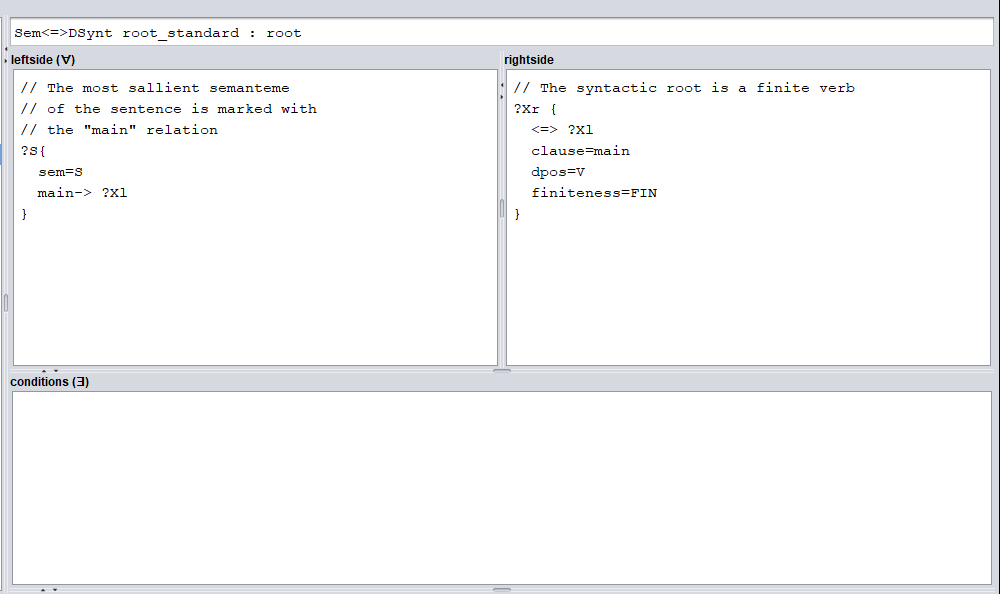
\includegraphics[width=1\textwidth, trim = {0cm 0cm 0cm 0cm},clip]{ch3/figs/grammaire.png}
	\caption{Règle créant la racine syntaxique}
	\label{fig:root}
\end{figure}

%%%%%%%%%%%%%%%%%%%%%%%%%%%%%%%%%%%%%%%%%%%%%%%%
% ---------G R A P H E S ------------------
%%%%%%%%%%%%%%%%%%%%%%%%%%%%%%%%%%%%%%%%%%%%%%%%

\subsubsection{Graphes}\label{entree-sortie}

Maitenant que nous avons fait un survol des dictionnaires et des modules de grammaires, il ne nous reste qu'à présenter les graphes. Dans un premier temps nous présenterons brièvement à quoi ressemble la construction d'un graphe en input. Puis nous montrerons à quoi ressemble les graphes en output.

L'input du réalisateur GenDR est un graphe sémantique \citep{mel2012semantics}\FL{\bf **** check ta biblio ****} où les prédicats sont liés à leurs arguments par des relations numérotées qui indiquent la position logique de l'argument. La figure~\ref{input} montre comment on construit un graphe sémantique dans MATE.

\begin{lstlisting}[language=XML, caption = Input sémantique, label=input]
structure Sem debt {
  S {
    owe {
    tense=PRES
    1-> Paul {class=proper_noun}
    2-> "\$500K" {class=amount}
    3-> bank {number=SG definiteness=DEF}}
    main-> owe } }
\end{lstlisting}

Toutefois, MATE offre aussi une version graphique pour encoder et visualiser le graphe sémantique (voir la figure \ref{fig:graphesem}).

\begin{figure}[htb]
	\centering
	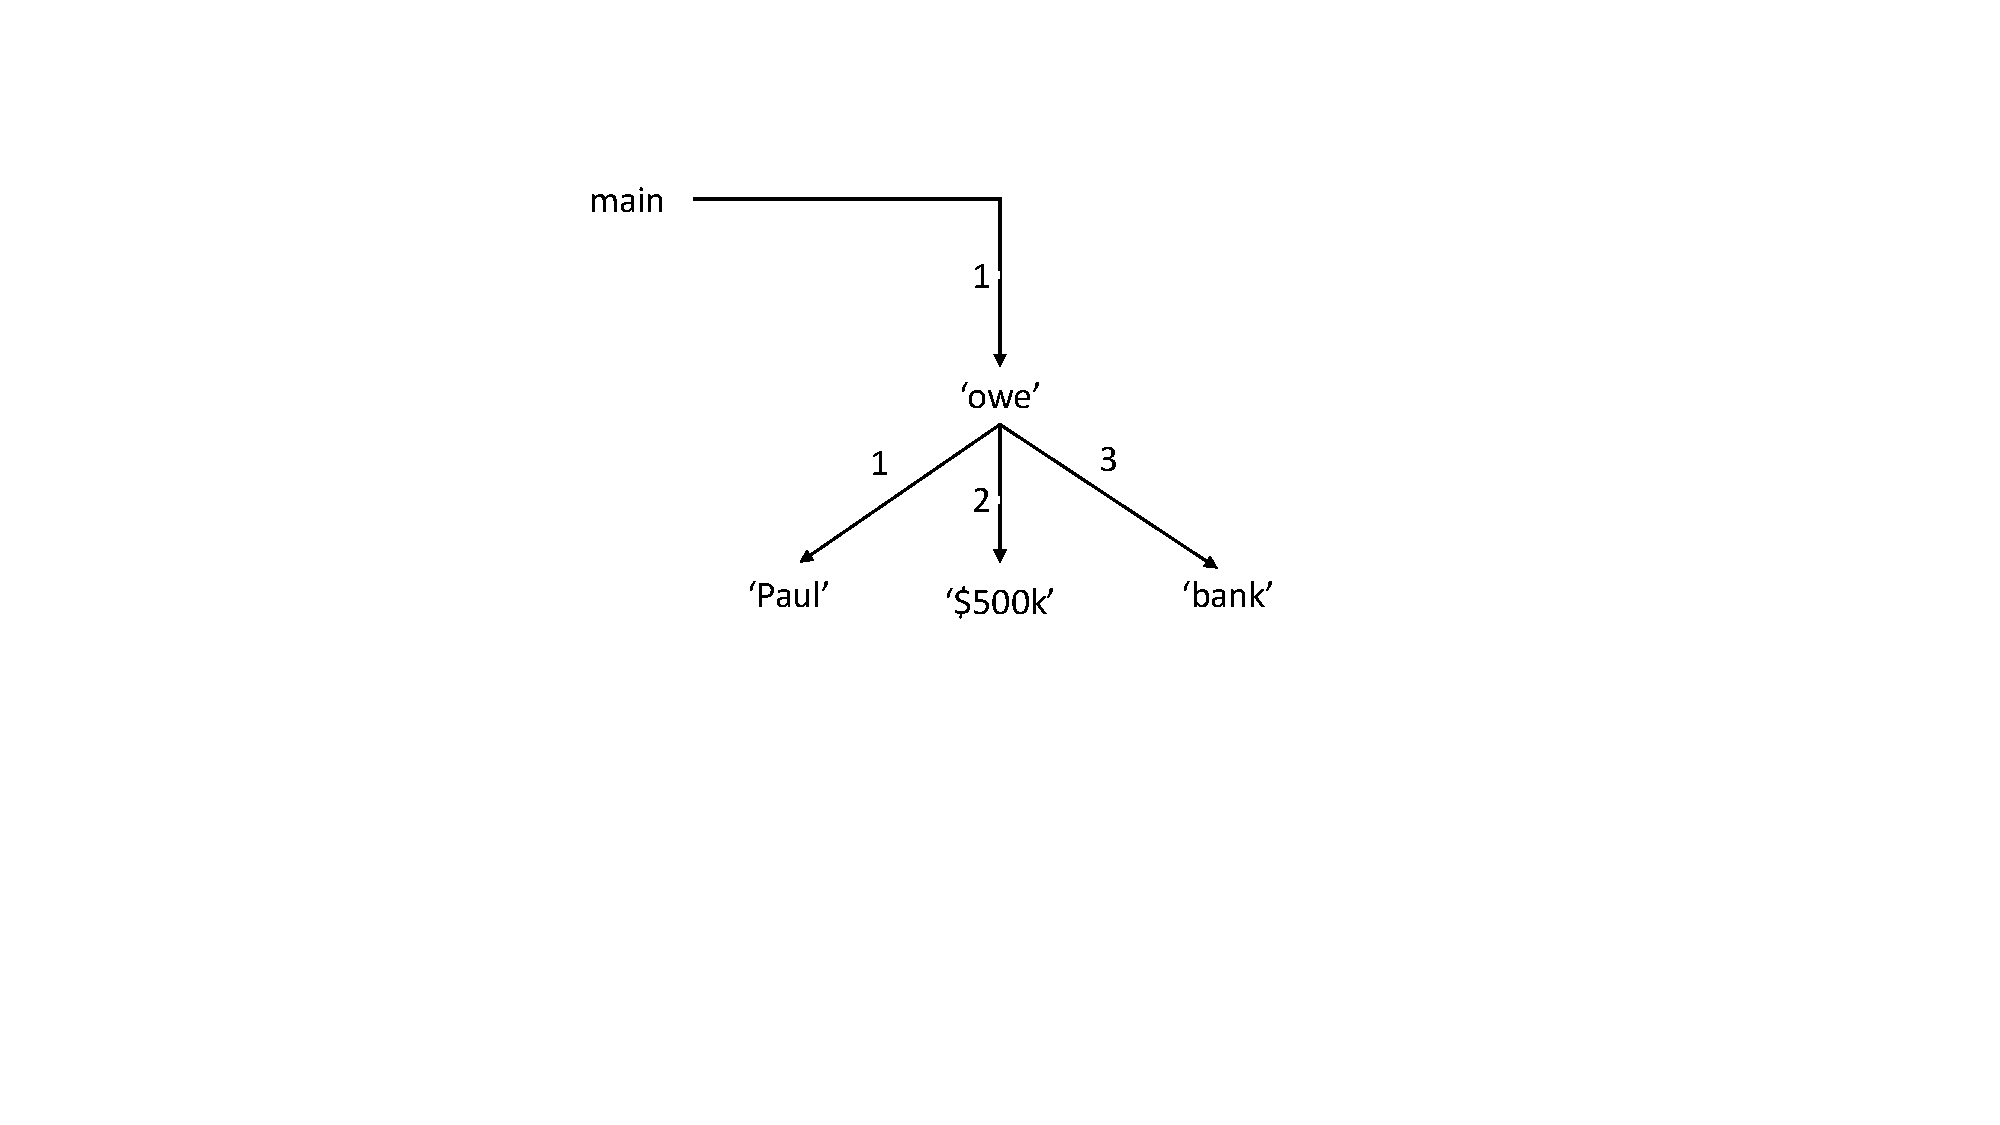
\includegraphics[width=1\textwidth, trim = {0cm 4cm 0cm 3cm},clip]{ch3/figs/owe_sem.pdf}
	\caption{Graphe sémantique en visuel}
	\label{fig:graphesem}
\end{figure}
\FL{trim le bas}

La section graphe de GenDR nous permet de construire les structures sémantiques d'input et de visualiser les transductions de graphes. Pour l'input donné en \ref{input}, GenDR réalise six structures syntaxiques de surface. Celles-ci peuvent être visualisées dans MATE grâce au module de graphes. La figure \ref{fig:realsurfex} est un exemple d'output visuel que fournirait MATE. 

\begin{figure}[htb]
	\centering
	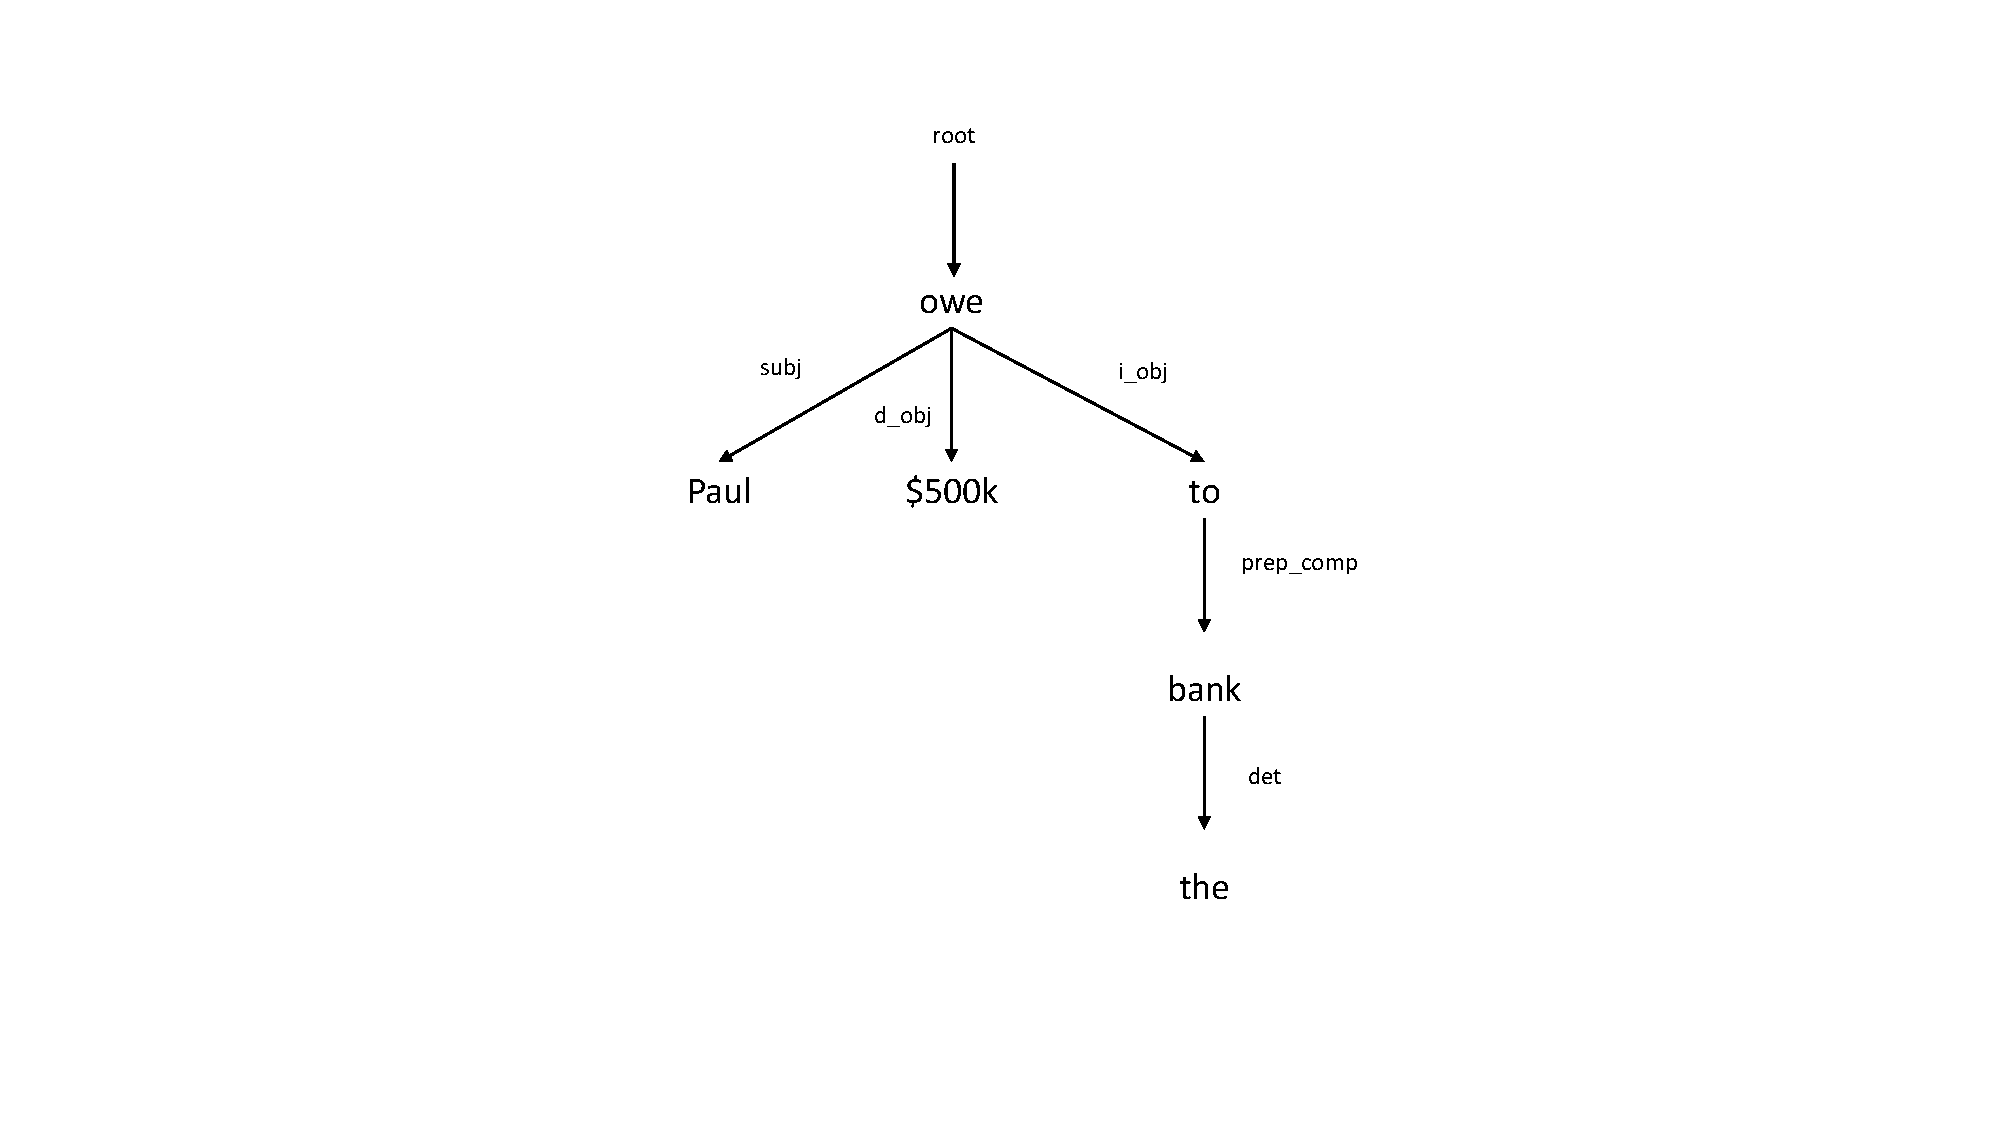
\includegraphics[width=1\textwidth, trim = {0cm 2cm 0cm 2cm},clip]{ch3/figs/realsurfex.pdf}
	\caption{Réalisation de surface}
	\label{fig:realsurfex}
\end{figure}

Toutefois, les modules de règles et de dictionnaires permettent en réalité de réaliser de six arbres syntaxiques superficiels (grâce aux mécanismes de paraphrasage). Nous les présentons à la figure \ref{fig:6realsurf}. Dans cette figure, les arbres de dépendances ont été linéarisés pour faciliter la compréhension du lecteur. Dans les faits, les arbres générés en output ne sont pas linéarisés et ils ressemblent à ceux de la figure \ref{fig:realsurfex}.

\begin{figure}[htb]
	\centering
	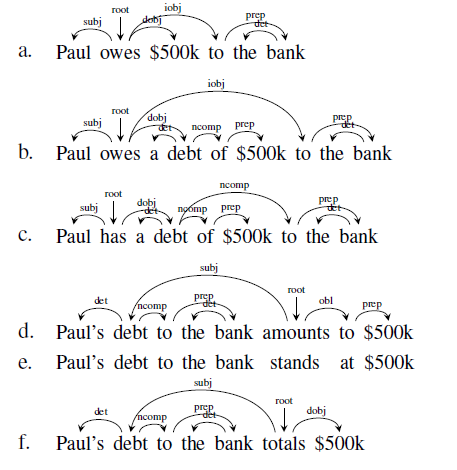
\includegraphics[width=0.5\textwidth, trim = {0cm 0cm 0cm 0cm},clip]{ch3/figs/exemples_real.png}
	\caption{Six réalisations syntaxiques de surface \citep{lareau18}}
	\label{fig:6realsurf}
\end{figure}
\FL{évite les captures d'écran si tu peux}

Si on souhaite une réalisation linéarisée et fléchie,  il faut utiliser un réalisateur de surface. C'est exactement dans ces contextes, que les réalisateurs de surface comme SimpleNLG ou JSreal \cite{DaoustJSREALTextRealizer2015}\cite{MolinsJSrealBBilingualText2015}\cite{GattSimpleNLGRealisationEngine2009} entrent en jeu. Au lieu de mettre des efforts à réaliser le texte jusqu'à la fin, GenDR concentre ses efforts à effectuer des tâches en amont. L'arborisation et la lexicalisation sont principalement les deux tâches où GenDR se démarque des autres réalisateurs. Nous les expliquerons en détail dans la section \ref{secsemsynt}.

%%%%%%%%%%%%%%%%%%%%%%%%%%%%%%%%%%%%%%%%%%%%%%%%%%%%%%%%%%%%%%%%%%%%%%%%%%%%%
% --------- I N T E R F A C E   S É M A N T I Q U E- S Y N T A X E ---------
%%%%%%%%%%%%%%%%%%%%%%%%%%%%%%%%%%%%%%%%%%%%%%%%%%%%%%%%%%%%%%%%%%%%%%%%%%%%%

\section{Interface sémantique-syntaxe en TST}\label{secsemsynt}

Dans la présente section, nous décrirons l'interface sémantique-syntaxe dans le cadre de la \ac{TST}. Plus précisément, nous décrirons deux processus nécessaires au passage de la sémantique à la syntaxe: l'arborisation et la lexicalisation. Pour mieux comprendre ce que sont ces procédés, nous ferons un très bref retour sur la \ac{TST}. 

La \ac{TST} vise la modélisation formelle de la correspondance entre les \emph{Sens} et les \emph{Textes} \citep{PolgueretheorieSensTexte1998}.\FL{melcuk67,97} La figure \ref{fig:modeletst}, qui vient de \cite{PolgueretheorieSensTexte1998}, présente comment fonctionnent ces modèles. Elle illustre le fait qu'un modèle Sens-Texte est une machine virtuelle qui prend en entrée des représentations sémantiques d'énoncés et génère un ensemble de paraphrases permettant d'exprimer le Sens donné en entrée. 

\begin{figure}[htb]
	\centering
	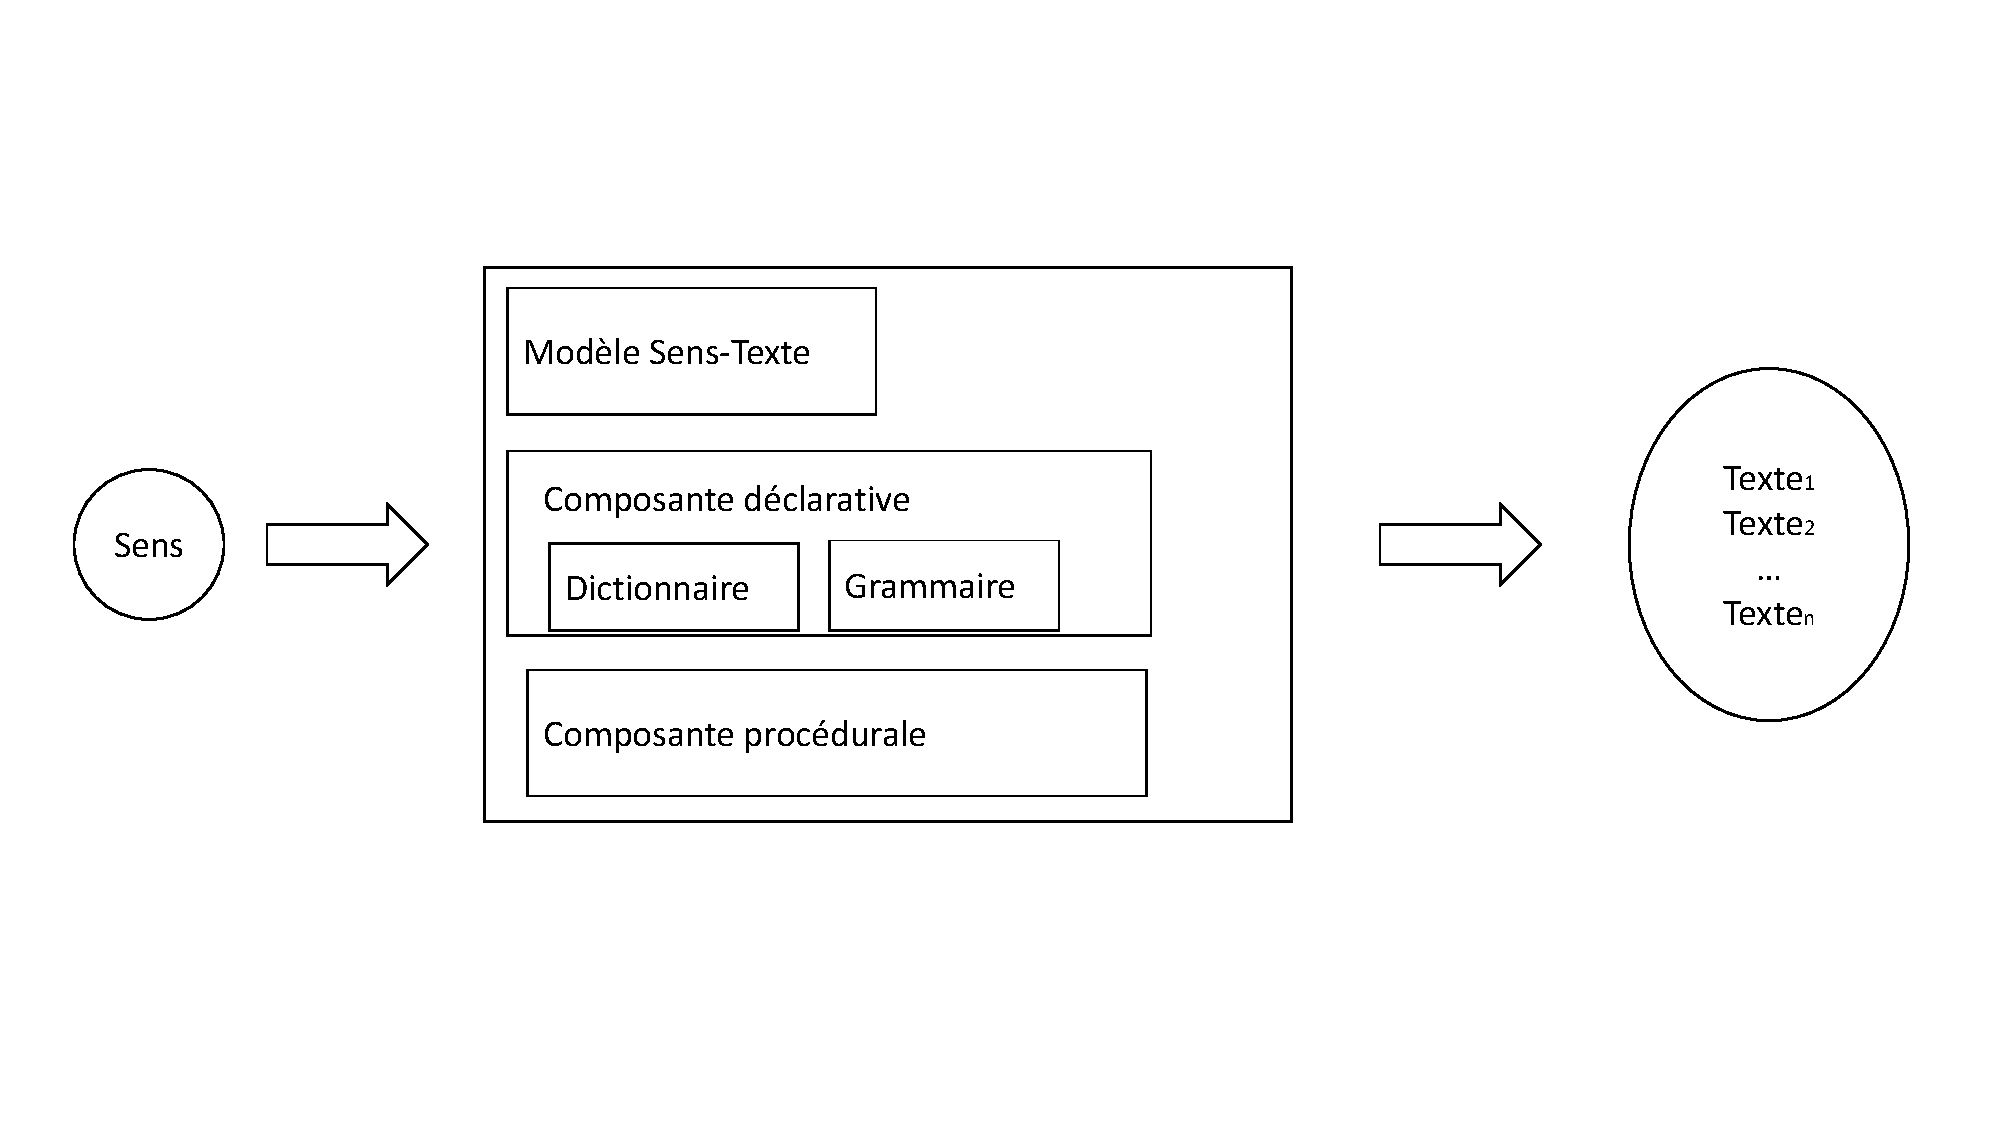
\includegraphics[width=1\textwidth, trim = {0cm 4cm 0cm 4cm},clip]{ch3/figs/polguere1.pdf}
	\caption{Structure d'un modèle Sens-Texte \citep{PolgueretheorieSensTexte1998}}
	\label{fig:modeletst}
\end{figure}
\FL{trim bien les figures importées, tu laisses trop d'espace avant et après les figures}

Concrètement, la figure \ref{fig:modeletst} démontre comment on passe de la figure \draft{2.4} (qui représente le Sens) à la figure \draft{2.6} (qui représente le Texte). Pour se rendre au texte final, le Sens traverse de nombreux niveaux de représentations. La figure \ref{fig:processustst} démontre les niveaux de représentations que l'input doit traverser succesivement, puis en parallèle comment on \draft{représente ces représentations} au cours de la réalisation.

\begin{figure}[htb]
	\centering
	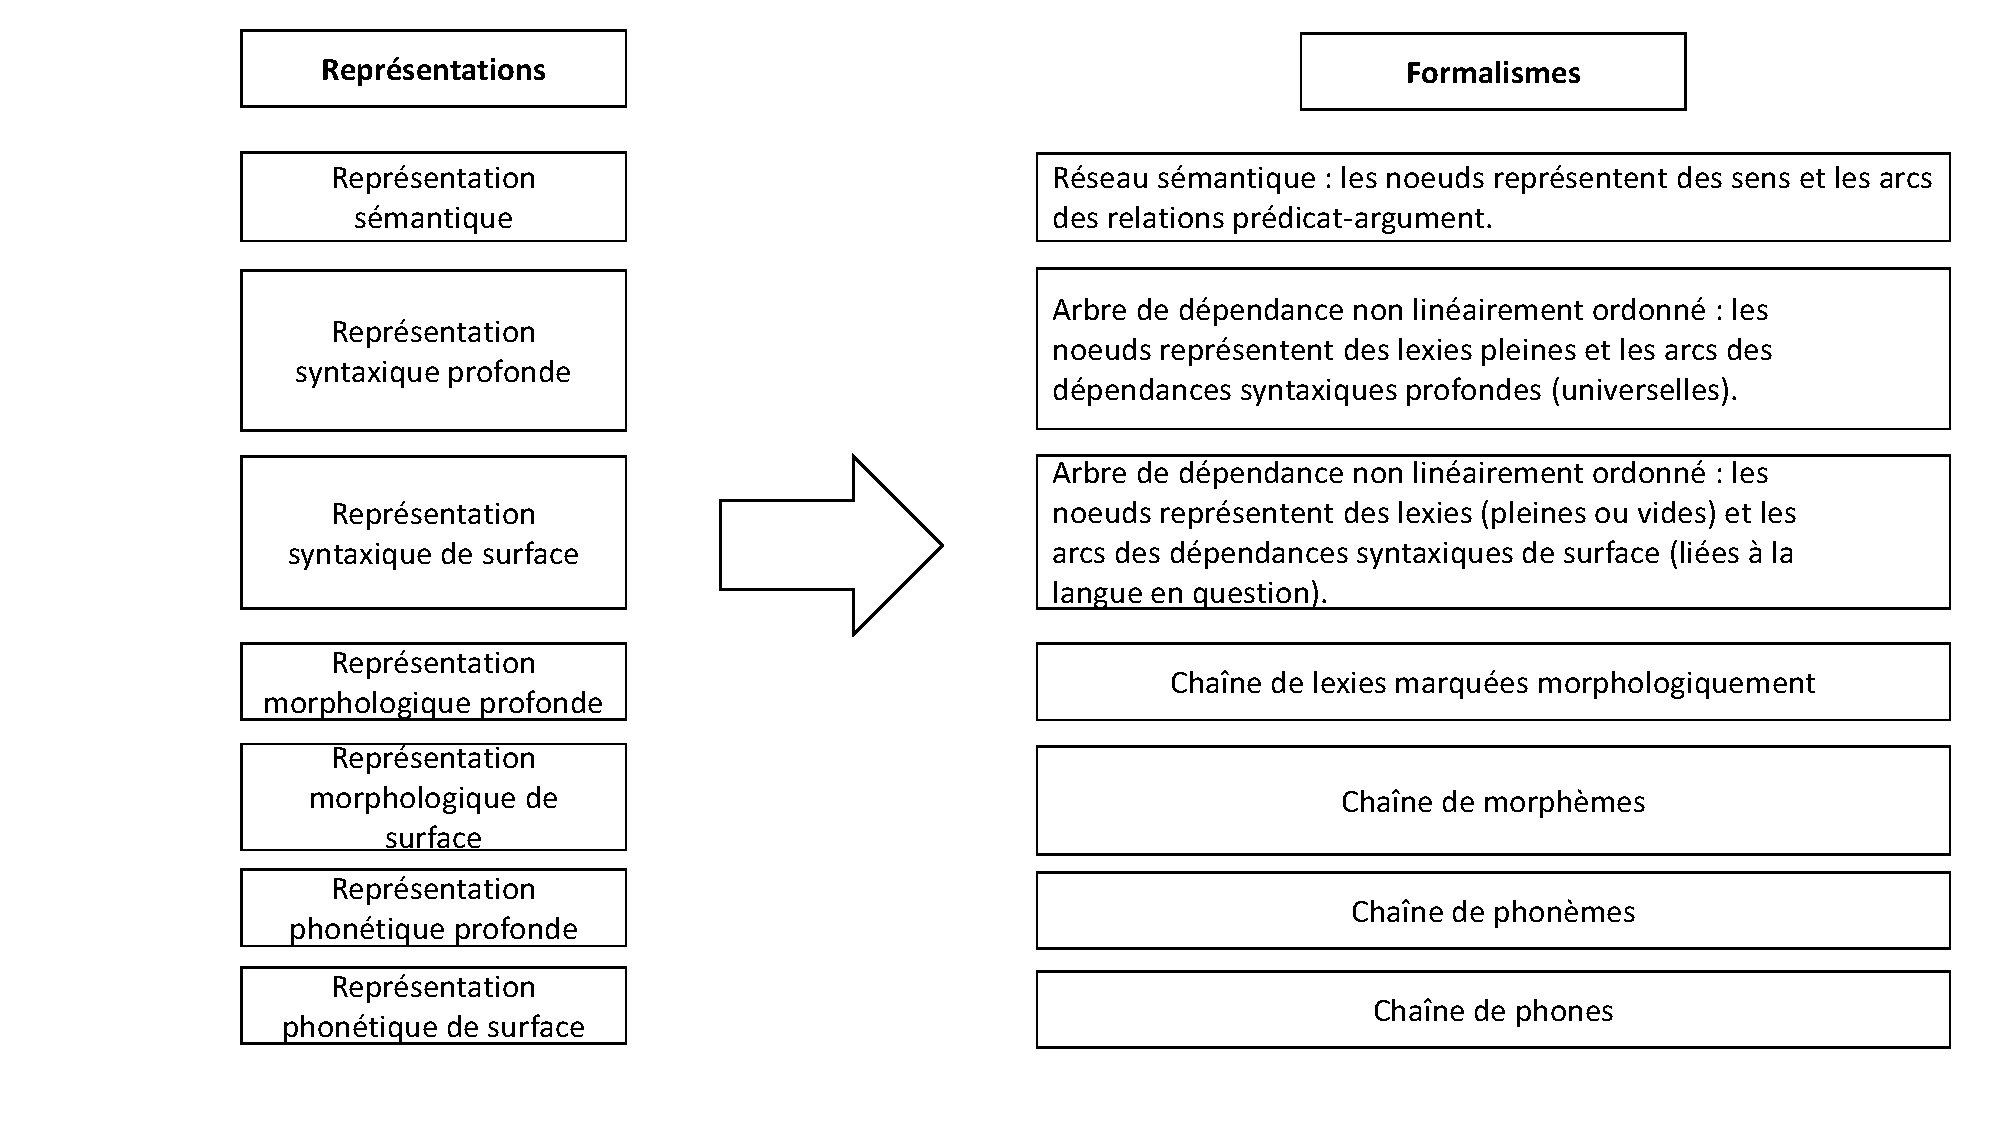
\includegraphics[width=1\textwidth, trim = {0cm 0cm 0cm 0cm},clip]{ch3/figs/polguere2.pdf}
	\caption{Processus d'un modèle Sens-Texte \citep{PolgueretheorieSensTexte1998}}
	\label{fig:processustst}
\end{figure}

%%%%%%%%%%%%%%%%%%%%%%%%%%%%%%%%%%%%%%%%%%%%
% ---------T H É O R I Q U E  ------
%%%%%%%%%%%%%%%%%%%%%%%%%%%%%%%%%%%%%%%%%%%

\subsection{Arborisation théorique}\label{arbo}

\FL{est-ce que cette division entre théorie et implémentation est vraiment utile? en théorie, y a pas vraiment d'ordre entre les opérations, donc en fait ta présentation ici suit plutôt la même structure que l'implémentation}

Comme GenDR n'utilise que trois niveaux de représentations, nous n'expliquerons que les processus pertinents pour ce système. Nous commencerons par l'arborisation, qui est le passage de la représentation sémantique à la représentation syntaxique profonde.

Selon la \ac{TST}, la structure syntaxique d'un énoncé représente l'ensemble des liens de dependances fonctionnelles qui existent entre les unités lexicales de cet énoncé \citep{melcuk1988}. On représente formellement ces structures syntaxiques par des arbres de dépendances. Cette approche syntaxique provient de \cite{TesniereElementssyntaxestructurale1965}\FL{check ta biblio, Fourquet est pas auteur} qui est le premier à l'avoir théorisée.

Formellement, le passage de la RSém \FL{acronyme: \lstinline!ac\{RSem\}!, check dans lng-acro-fr.sty} à la RSyntP se nomme l'arborisation. Elle est ainsi nommée  parce qu'on cherche à arboriser la RSém pour qu'il en résulte un arbre de dépendance profond. Ce passage est effectué via des règles de correspondance sémantiques.

Pour que l'arborisation se fasse correctement, il faut que la racine de l'arbre en construction corresponde à un noeud sémantique identifié comme étant le plus saillant. La détermination de la racine correspond au processus de hiérarchisation de \cite{PolguereStructurationmisejeu1990}. On l'appelle ainsi car la racine est le noeud qui domine tous les autres de l'arbre syntaxique profond. Une fois que c'est fait, on va trouver le lexème qui peut satisfaire les contraintes de la racine. Il faut que le lexème sélectionné corresponde à l'unité sémantique identifiée comme la plus saillante.\FL{déjà dit, reformule} Le lexème doit aussi satisfaire des contraintes comme la partie du discours ou la finitude. Généralement, dans les langues européennes, on a ces contraintes sur la racine puisque ce sont le plus souvent les verbes qui contrôlent les énoncés. En lexicalisant le noeud, on va \draft{simultanément}\FL{simultanément? je pense pas, plutôt après, non?} ajouter les arcs qui en dépendent. Ceux-ci correspondent aux arguments liés à ce prédicat dans la RSém. Comme Polguère le dit: ``chaque arc est considéré successivement dans l'ordre du parcours, puis est traduit en une micro-structure syntaxique profonde grâce aux règles de correspondance sémantique de la grammaire.'' \citep[p.~273]{PolguereStructurationmisejeu1990}.\FL{check dans le code comment générer cette référence avec num de page}

Une fois que l'arborisation est complétée, l'arbre de dépendance profond \draft{transitera} vers le niveau syntaxique de surface, ce qui implique les opérations suivantes. D'abord, faire le calcul des relations syntaxiques de surface. Ainsi, la relation I deviendra sujet, la relation II deviendra complément d'objet direct, etc. De plus, on incorpore les lexies vides (prépositions, déterminants, etc.) à ce stade et on opère la pronominalisation.

\FL{t'as besoin de faire plus d'\scare{aggrégation} quand tu écris. tu fais souvent qqch comme: X fait Y. Y est Z., alors que tu pourrais faire: X fait Y, qui est Z. ou qqch du genre. faut développer ça, c'est ce qui rend un texte plus fluide et plus dense. regarde les modifs que j'ai faites au texte, tu verras que c'est souvent des passages du genre}

\subsection{Lexicalisation théorique}

Tel que nous l'avons montré dans la figure \draft{figure dans MARQUIS}, la lexicalisation se produit entre la RSém et la RSyntP \citep{PolguereStructurationmisejeu1990}.\FL{récupère les citations sur lexicalisation de Florie, notamment les travaux de Wanner} Concrètement, il s'agit de la \draft{correspondance} entre une unité sémantique et les lexies qu'elle contrôle. La \draft{correspondance}\FL{ici, par exemple, tu peux fusionner ces deux phrases} est inscrite dans le dictionnaire sémantique et lexical. La lexicalisation est ainsi étroitement liée à l'arborisation car ces deux étapes se produisent lors du passage de la RSém à la RSyntP. La construction de la représentation syntaxique profonde est une conséquence de l'arborisation des arcs de la RSém et de la lexicalisation des unités sémantiques de cette RSém. Le tout résulte en un arbre de dépendance lexicalisé. Comme nous l'avons vu dans la figure \draft{au début}, le passage de \sem{owe} à \lex{owe} et \lex{debt} \draft{représente la lexicalisation.}\FL{reformule}

%%%%%%%%%%%%%%%%%%%%%%%%%%%%%%%%%%%%%%%%%%%%%%%%%%%%%
% --------- C O M P U T A T I O N N E L L E  ------
%%%%%%%%%%%%%%%%%%%%%%%%%%%%%%%%%%%%%%%%%%%%%%%%%%%%

\section{Arborisation et lexicalisation computationnelle}\label{secarbolex}

Maintenant que nous avons présenté le côté théorique de l'interface sémantique-syntaxe, nous exposerons comment ces mécanismes se traduisent d'un point de vue computationnel dans GenDR.

\subsection{Arborisation computationnelle}
La première étape du processus d'arborisation dans GenDR est la même que celle que nous avons expliquée d'un point de vue théorique.\FL{donc aussi bien en faire une seule section, fusionne-les} Il faut créer la racine de l'arbre qui correspond au noeud le plus saillant de la RSém. Pour faire cela, nous devons indiquer le noeud le plus saillant dans la structure d'input (voir \draft{figure x}). L'arbre syntaxique profond est construit avec un algorithme top-down qui ressemble beaucoup à celui qu'utilisent MARQUIS et FORGe puisqu'ils sont aussi des tenants de la TST.\FL{ou plutôt parce que FORGe et GenDR l'ont hérité de MARQUIS, qui est inspiré de \cite{PolguereStructurationmisejeu1990}}

\subsubsection{Règles de base pour l'arborisation}
L'arborisation dans GenDR se fait en trois étapes.

\begin{enumerate}
  \item Création de la racine.
  La première règle appliquée est \emph{root\_standard}. Elle construit la racine de l'arbre syntaxique à partir du noeud principal de la structure sémantique. À cette étape, la racine n'est pas étiquetée par un lexème encore (le noeud est vide), mais on peut lui imposer des contraintes, par exemple pour exiger un verbe à l'indicatif. Cette règle ne s'applique qu'une seule fois par réalisation.

  \item Lexicalisation de la racine.
  Une fois que la racine a été créée et contrainte, on applique une règle de lexicalisation. Cela permet au système de fouiller dans les dictionnaires pour trouver un lexème qui correspondra au sens demandé tout en respectant les contraintes imposées.

  \item Application des règles actancielles.
  Une fois que le noeud racine est lexicalisé, GenDR regarde dans le patron de régime de la racine pour savoir comment faire le passage des arcs sémantiques aux arcs syntaxiques. Ceux qui partent du noeud sémantique vers ses arguments seront réalisés comme des actants syntaxiques. Tandis que les arcs qui pointent vers le noeud seront réalisés comme des modificateurs. Bref, les règles qui sont utilisées à cette étape créent de nouveaux noeuds et de nouveaux arcs en partance de la racine. Ces noeuds se font imposer des contraintes par le patron de régime du gouverneur (la racine) et les lexies qui satisferont ces contraintes pourront être lexicalisés. C'est ainsi qu'on retourne à la seconde étape pour lexicaliser ces noeuds. Puis cycliquement, nous retournons à la troisième étape puisque de nouveaux noeuds lexicalisés amènent leur patron de régime avec eux. Et ce jusqu'à ce que le graphe sémantique soit complètement réalisé en surface profonde. Les règles sémantiques qui s'occupent de cela sont: \emph{actant\_gp}, \emph{actant\_guess}, \emph{attr\_lex}.\FL{à ce stade-ci on a pas vu la liste des règles donc ça sert pas à grand-chose de les nommer}
\end{enumerate}

\subsection{Lexicalisation computationnelle} \FL{fusionner avec théorie?}

\FL{mentionne que tu reprends essentiellement \cite{lareau18} ici}

La lexicalisation dans GenDR implique trois niveaux de représentations (RSém, RSyntP et RSyntS) et se fait en deux étapes. La lexicalisation profonde est la première des deux étapes. Il s'agit de faire correspondre une unité sémantique à une unité lexicale profonde. Cette phase introduit des lexies pleines de sens. S'ensuit la lexicalisation de surface qui consiste à introduire les mots fonctionnels et les lexies de surface. La phase de lexicalisation s'opère grâce à des ressources lexicales: des dictionnaires et des règles de lexicalisation. Ainsi, la sélection de l'unité lexicale profonde pour réaliser l'unité sémantique fournie en input se fait en consultant les dictionnaires lexicaux. Dans GenDR, nous deux dictionnaires servant contribuant à l'étape de lexicalisation. Nous avons d'abord, le dictionnaire sémantique, puis le dictionnaire lexémique et un dictionnaire de fonction lexicale. Il s'agit de ceux qui ont été présentés en \ref{dictio}. \draft{En ce qui concerne les règles.} Nous décrirons, dans cette section, quelques règles de lexicalisation de base. Nous omettrons les règles de lexicalisation complexes (collocations, locutions, etc.) car ce n'est pas le propos de ce mémoire. Pour plus d'informations concernant celles-ci, voir \cite{lambrey15,LambreyImplementationcollocationspour2017,dubinskaite17,lareau18}.\FL{relire ce paragraphe}

\textbf{Les lexicalisations simples}
sont traitées par la règle \emph{lexicalization\_standard}. Cette règle prend une unité sémantique donnée dans un graphe sémantique et vérifie dans le dictionnaire sémantique quelles sont les correspondances lexicales de ce sémantème (tel que démontré en \ref{semanticon}). Puis le système récupère toutes les lexicalisations possibles de l'unité sémantique. S'ensuit la sélection de l'unité lexicale. Pour ce faire, GenDR s'assure que la partie du discours profonde de la (ou les) lexie(s) correspond à celle qui est demandée sur le noeud contraint dans l'arbre syntaxique profond en construction. Effectivement, si la lexie satisfait les contraintes du noeud, alors GenDR permet la lexicalisation. L'arbre syntaxique profond sera désormais doté d'un noeud consommé par cette lexie choisie. D'ailleurs, c'est ce mécanisme qui permet le paraphrasage. Puisque le système créera autant d'arbres syntaxiques profonds qu'il y a de lexies possibles pour un noeud donné. 

\textbf{Lexicalisation de classes}
Les classes comme les nombres, les montants, les noms propres ou les acronymes ont une règle de lexicalisation particulière qui se charge des unités sémantiques que nous ne voulons pas dans nos dictionnaires sémantiques et lexicaux parce qu'elles sont trop nombreuses et que leur comportement est prévisible. Pour déclencher l'application de cette règle, on précise dans la structure d'input à quelle classe le sémantème appartient. Les traits lexicaux (DPOS\FL{est-ce que c'est clair pour le lecteur, dpos?}, etc.) de ces classes sont encodés dans le lexicon.

\textbf{Lexicalisation de secours}
Les règles de lexicalisation de secours permettent à GenDR de lexicaliser une unité sémantique ou lexicale dont il n'a pas les informations. Puisque le système possède les 1\,500 lexies les plus fréquentes de l'anglais, il est évident que certaines lexies ou sémantèmes manqueront à l'appel. Pour remédier à la situation, il y a deux mécanismes. D'abord, si le sémantème dans l'input existe sous la même forme dans le \emph{lexicon}, alors le système va lexicaliser le sémantème avec ce lexème. Cela a comme conséquence qu'on n'a pas besoin d'inscrire le sémantème dans le \emph{semanticon} s'il n'y a qu'une lexicalisation possible de celui-ci (cela permet de sauver du temps). Cependant, si le sémantème ne figure pas dans le \emph{lexicon}, alors le système suppose que l'étiquette de l'unité sémantique est la même que l'unité lexicale, et s'il y a des contraintes sur le noeud d'arrivée, alors le système suppose que l'unité lexicale ainsi créée satisfait les contraintes. Les lexèmes devinés seront mis en évidence dans la structure d'output afin qu'on ait une trace qu'une règle de lexicalisation de secours a été employée.
	
\textbf{Lexicalisation grammaticale}
Alors que les règles de lexicalisation précédentes prenaient place entre la RSém et la RSyntP, les règles de lexicalisation grammaticale prennent place au niveau syntaxique de surface (RSyntS) et introduisent des lexèmes fonctionnels. Il y a des règles qui introduisent les lexèmes exprimant des sens grammaticaux comme les auxiliaires et les déterminants. Ces règles sont déclenchées par la présence de sens grammaticaux dans les structures d'input (voir la figure \draft{exemple}). Ces lexèmes existent en syntaxe profonde, mais on ne les voit pas sous forme de noeuds, mais plutôt sous forme de traits sur les noeuds lexicaux. Comme ces mots appartiennent à une classe fermée et qu'ils sont peu nombreux et souvent spécifiques à une langue, ce sont des règles particulières qui traitent ces lexicalisations dans chaque module de langue. Puis, il y a des règles de lexicalisation grammaticales qui s'occupent des lexèmes régis (comme les prépositions). Ces lexèmes régis sont introduits en syntaxe comme des noeuds supplémentaires entre un gouverneur et son actant. Ils sont donc encodés dans le patron de régime du gouverneur.

%%%%%%%%%%%%%%%%%%%%%%%%%%%%%%%%%%%%%
% --------- E X E M P L E ---------
%%%%%%%%%%%%%%%%%%%%%%%%%%%%%%%%%%%%%

\section{Exemple}\label{secexemple}

Pour illustrer le fonctionnement des règles et des dictionnaires que nous avons présentés, nous décortiquerons la réalisation profonde de l'exemple vu à la figure~\ref{input}.

\subsection{1ère phase: RSém à RSyntP}
Cette section illustre les étapes successives qui ont permis à GenDR de passer de la \ac{RSém} à la \ac{RSyntP}. Il s'agit de l'arborisation profonde et de la lexicalisation profonde.

\subsubsection{Application de la règle \emph{root\_standard}}
La règle crée un noeud vide qui sera la racine de l'arbre à construire. Ce noeud est contraint par deux traits et il demande un verbe fini. La figure \ref{fig:rootstand} illustre la création du noeud non-étiqueté.
\begin{figure}[htb]
	\centering
	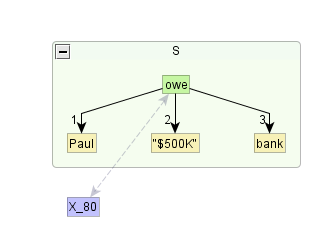
\includegraphics[width=0.6\textwidth, trim = {0cm 0cm 0cm 0cm},clip]{ch3/figs/inspecteur_root.png}
	\vspace{-0.5cm}
	\caption{Application de \emph{root\_standard}}
	\label{fig:rootstand}
\end{figure}

\subsubsection{Application de la règle \emph{lex\_standard}}
Ensuite, on procède à la lexicalisation de la racine. Le sémantème \sem{owe} peut correspondre à deux lexèmes selon le \emph{semanticon}: \lex{owe} et \lex{debt}. GenDR va donc tenter de combler la racine avec ces deux lexèmes. Il peut lexicaliser la racine en choisissant \lex{debt} car ce nom commun est associé à des verbes supports. Mais il s'agit d'une lexicalisation complexe, donc et nous renvoyons le lecteur à \cite{lambrey15,LambreyImplementationcollocationspour2017,lareau18}, pour nous concentrer sur la lexicalisation simple avec le verbe \lex{owe}.

\begin{figure}[htb]
	\centering
	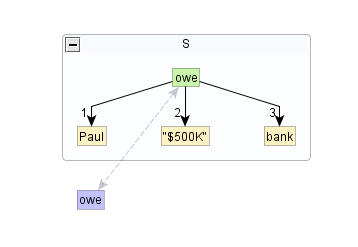
\includegraphics[width=0.7\textwidth, trim = {0cm 0cm 0cm 0cm},clip]{ch3/figs/lex_standard_root.png}
		\vspace{-0.5cm}
	\caption{Application de lex\_standard}
	\label{fig:lexstand1}
\end{figure}

\subsubsection{Application de la règle \emph{actant\_gp}}
Une fois que la racine est pourvue d'un lexème, l'application de la règle \emph{actant\_gp} est déclenchée. Pour chaque relation actancielle, le système puise dans le patron de régime de \lex{owe} et met en correspondance les actants sémantiques avec des actants syntaxiques. Dans l'input (figure~\ref{input})\FL{évite les labels comme ``input'' pour tes figures, t'es presque sûr d'avoir un doublon quelque part}, \sem{owe} possède trois actants sémantiques. Ils seront réalisés en actants syntaxiques en fonction de la diathèse imposée par \lex{owe} dans le \emph{lexicon}. Brièvement, la diathèse est la correspondance entre les actants sémantiques et syntaxiques.\FL{ça devrait venir beaucoup plus tôt, ça fait déjà un bout que tu parles de ça} Puis les noeuds au bout des arcs syntaxiques seront contraints en fonction des restrictions prévues par le patron de régime de \lex{owe} pour chacun de ses actants syntaxiques. Le patron de régime du verbe demande que deux de ses actants syntaxiques aient le trait dpos=N et qu'un ait dpos=Num. Nous élaborerons plus en détails sur les notions de patron de régime et diathèse à la section \ref{sectiongp}. \draft{\lstinline!(gp = {1=I 2=II 3=III} et (I={dpos=N} and III={dpos=N})!, et l'actant II est soit un montant ou un nombre (II={dpos=Num}).}

\begin{figure}[htb]
	\centering
	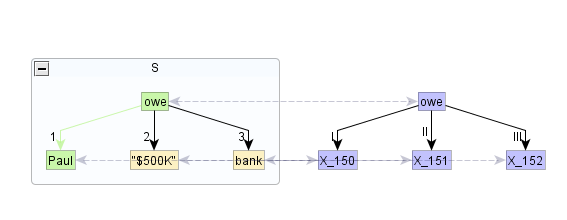
\includegraphics[width=1\textwidth, trim = {0cm 8mm 0cm 15mm},clip]{ch3/figs/actant_gp1.png}
	\caption{Application de actant\_gp}
	\label{fig:actantgp}
\end{figure}

\subsubsection{\draft{lex class et lex standard}}

Puisque nous avons maintenant de nouveaux noeuds non-étiquetés, il faut répéter la lexicalisation pour trouver les lexèmes correspondant aux entrées \sem{Paul}, \sem{bank} et \sem{\$500}. À cette étape, GenDR utilise deux règles de lexicalisation différentes: une règle de lexicalisation pour les classes(\emph{lex\_class}) et une règle de lexicalisation standard(\emph{lex\_standard}). Il utilise \emph{lex\_class} car \sem{Paul} et \sem{\$500} ont des traits \emph{class}\FL{dit explicitement class=propernoun, class=amount pour qu'on comprenne le passage où tu parles des entrées du lexicon} dans l'input sémantique. \draft{Elle} passe directement au \emph{lexicon}, puisque les sens ne sont pas décrits dans le \emph{semanticon}. Dans le \emph{lexicon} par contre, les classes sont décrites. En effet, les \emph{classes proper\_noun} et \emph{numeral} permettent l'application de la règle lex\_class et de lexicaliser \draft{paul et 500 piastres}. Les classes ont les informations de type dpos et autres traits grammaticaux. L'étiquette du noeud sémantique est directement copiée en syntaxe. on s'assure finalement que les contraintes de ces classes respectent les contraintes du noeuds généré par gp\_actant. Lorsque c'est le cas, la lexicalisation se produit. Les noms propres héritent des traits de la classe des noms, donc la dpos est là, puis les montants héritent des traits de la classe des nombres. Ensuite le système utilise \emph{lex\_standard} pour lexicaliser \sem{bank}. Le processus est le même que nous avons décrit pour la première occurrence de cette règle.\lex{bank} sera lexicalisé comme III actant syntaxique puisqu'il correspond au sens \sem{bank} et parce qu'il satisfait les contraintes du noeud imposées par la règle \emph{actant\_gp}.\FL{lisser ce paragraphe}

\begin{figure}[htb]
	\centering
	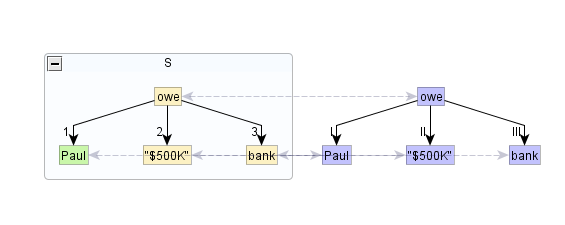
\includegraphics[width=1\textwidth, trim = {0cm 0cm 0cm 0cm},clip]{ch3/figs/lex_standard2.png}
	\caption{Application de lex\_standard}
	\label{fig:lexstand2}
\end{figure}

\FL{trim les figures}

\subsection{2ème phase: RSyntP à RSyntS}

\subsubsection{Application des règles de lexicalisation de surface}
On va chercher les lexicalisations de surface de chacune des unités lexicales avec les règles \emph{lex\_class} et \emph{lex\_lu}. La première se charge de lexicaliser en surface les unités de type classe et la seconde les unités normales. \FL{\ldots}

\begin{figure}[htb]
	\centering
	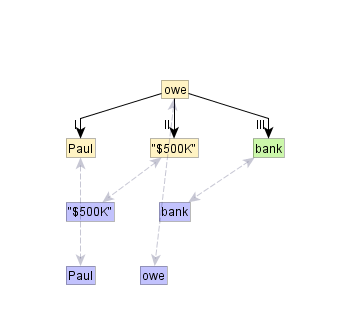
\includegraphics[width=0.7\textwidth, trim = {0cm 0cm 0cm 0cm},clip]{ch3/figs/rsyntslexicalisation1.png}
	\caption{Application de lex class et lex lu}
	\label{fig:lexsurf}
\end{figure}

\subsubsection{Application des règles actancielles de surface}
Ensuite, les règles actancielles de surface s'appliquent. Concrètement, ces règles remplacent les étiquettes des arcs de l'arborisation profonde (I, II, III,...) par des étiquettes de syntaxe de surface (sujet, objet direct, objet indirect,...). Ces étiquettes de surface sont encodées dans le patron de régime du verbe qui gouverne les actants syntaxiques. Ainsi, la relation subjectale est réalisée par la règle \emph{actant\_subj}. Qui réalise la relation entre le sujet et le verbe. Cette information est encodée dans le gp du verbe \lex{owe} qui hérite des traits de la classe verb\_dit. Celle-ci hérite des traits de la classe verb\_dt qui hérite des traits de la classe verb. C'est dans celle-ci que se trouve l'information nécessaire à l'application de la règle \lstinline!gp = { I = { dpos = N rel = subjective } } !. Ainsi, on voit encore comment le dictionnaire et les règles sont inter-reliés. Pour que la règle actant\_subj s'applique au sujet de la structure, elle va regarder dans la dictionnaire à quel actant syntaxique elle doit faire le lien. Elle ne prend que l'actant syntaxique qui précise la relation subjective.

Les mêmes phénomènes s'appliquent ensuite pour les règles \emph{actant\_dir} et \emph{actant\_prep}. Toutefois, la règle \emph{actant\_prep} diffère des deux autres règles actancielles car elle crée un noeud intermédiaire en syntaxe de surface pour accueillir le lexème fonctionnel \lex{to} qui est nécessaire à la bonne formation de la phrase. La nature de la préposition est encodée dans le gp du verbe ainsi \lstinline! gp = {III = { dpos = N  rel = indir_objective  prep = to }  }!.

\subsubsection{Application de la règle des déterminants}

La règle \emph{det\_def} ajoute les déterminants aux lexèmes en fonction de leur définitude. Parmi les règles que nous avons présenté, c'est la seule règle de GenDR qui est propre à l'anglais. Elle lexicalise \lex{the} puisque l'unité sémantique \sem{bank} était marquée par le trait défini dans la structure d'input.

La figure \ref{fig:syntsurf} démontre l'application simultanée des règles actancielles et de la règle des déterminants.

\begin{figure}[htb]
	\centering
	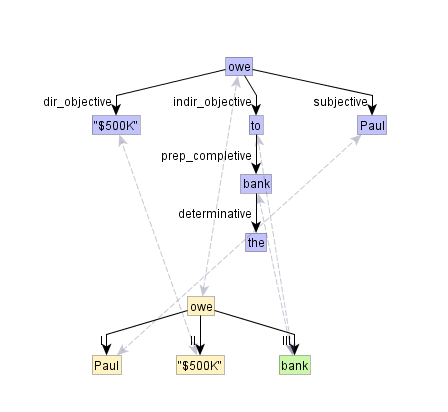
\includegraphics[width=0.7\textwidth, trim = {0cm 0cm 0cm 0cm},clip]{ch3/figs/rsynts_syntactisation.png}
	\caption{Application de subj,dir,prep et det}
	\label{fig:syntsurf}
\end{figure}

%%%%%%%%%%%%%%%%%%%%%%%%%%%%%%%%%%%%%%%%%%%%%%%%
% --------- P R O B L É M A T I Q U E ---------
%%%%%%%%%%%%%%%%%%%%%%%%%%%%%%%%%%%%%%%%%%%%%%%%

\section{Problématique}\label{problema}

La démonstration précédente montre que GenDR modélise bien les phénomènes linguistiques profonds. Toutefois, le dictionnaire lexical de ce système ne couvre que les 1\,500 lexies les plus fréquentes (en anglais et en français). Pour offrir une couverture plus large, il faudrait que GenDR possède beaucoup plus d'entrées lexicales, en particulier les verbes, car ce sont eux qui contrôlent la structure de la phrase:

\begin{quote}
In particular, since verbs often convey the main idea of a sentence, such a resource must represent verb meanings. These require a particularly precise and well deffined representation that captures both their predicate-argument structure as well as their semantic content.
\end{quote}
\vspace{-\baselineskip}
\hfill
\cite{SchulerVerbnetBroadcoverageComprehensive2005}

Nous sommes en accord avec cette déclaration, tout comme \cite{Korhonenlargesubcategorizationlexicon2006} et \cite{MESSIANT08.142}, qui suggèrent aussi que la modélisation informatique des langues naturelles passe par des ressources lexicales décrivant les comportements syntaxiques des lexèmes. Nous pensons qu'une ressource comme GenDR bénéficierait grandement d'une large couverture des verbes dans le cadre de la réalisation profonde. Parmi les 1\,500 lexies de l'anglais, 500 sont des verbes. Cela est non-négligeable mais, il est clair que GenDR gagnerait en couverture linguistique s'il se dotait d'une ressource lexicale lui permettant de traiter plus de verbes. C'est la raison d'être de ce mémoire. Nous tentons d'intégrer à GenDR un dictionnaire décrivant les comportements syntaxiques des verbes.

\section{Patrons de régime}\label{sectiongp}

\draft{refaire tout ce paragraphe:
Pour mieux comprendre l'utilité d'un tel dictionnaire, il faut expliquer ce sont les patrons de régime. Dans l'exemple plus haut, nous avons vu comment les patrons de régime permettaient l'arborisation. Les patrons de régime décrivent les cooccurrences syntaxiques des unités lexicales \citep{MilicevicSchemaregimepont2009}. La cooccurrence de la lexie avec ses actants. Autrement dit les sujets et objets des verbes, les compléments du nom. Ceux-ci correspondent aux actants syntaxiques de surface. Le patron de régime encode des relations plus profondes comme les actants syntaxiques profonds. Les patrons de régime d'une lexie correspondent à l'ensemble des constructions syntaxiques dont la lexie est la gouverneure. Les actants syntaxiques en sont ses dépendants. On les encode dans un dictionnaire car les patrons de régime des lexies ne sont généralement pas prévisibles. Effectivement, on ne peut pas prédire les patrons de régime des unités lexicales d'une langue. D'ailleurs, même des verbes sémantiquement proches ne possèderont pas nécessairement les mêmes constructions syntaxiques ex de Milicevic p. 95( se souvenir de X , mais se rappeler X ). Le nombre d'actant n'est pas prévisible non plus en regardant l'unité lexicale à partir de son sens. 

Puisque les arguments sélectionnés par une lexie sont généralement idiosyncratiques, on encode ces comportements syntaxiques dans des dictionnaires.

les GP encodent la diathèse (correspondance entre les actants sémantiques d'une lexie et ses actants syntaxiques profonds) et la réalisation des actants (I à sujet II objet direct, indirect, ou oblique). La diathèse peut soit être triviale (1 pour I, 2 pour II, etc.) ou pas (1 -II et 2-I)

Le patron de régime d'une lexie encode les correspondances entre ses actants (au niveau sémantique, syntaxique profond et syntaxique de surface), les moyens morpho-syntaxiques d'expressions des actants et les restriction sur les actants.

Plus tôt dans le chapitre nous avions parlé de l'interface sémantique-syntaxe et de l'importance des règles sémantiques qui font la transition entre Rsem et RSyntP. Le rôle le plus important du GP est de fournir l'information nécessaire au passage de la sem à la synt lors des opérations de lexicalisation et d’arborisation. 
}
\begin{quote}
Comme le choix lexical détermine le choix des constructions syntaxiques possibles (la lexie sélectionnée « amène » avec elle son régime) et vice-versa (le choix d’une structure impose certains choix lexicaux), on peut dire que c’est le schéma de régime qui, au sein d’un MST, fait le pont entre le lexique et la grammaire.
\end{quote}
\vspace{-\baselineskip}
\hfill
\cite[p.~105]{MilicevicSchemaregimepont2009}

\draft{faire une meilleure transition ici}
GenDR bénéficierait énormément d'un dictionnaire de patron de régime.\FL{tu l'as dit} Notamment parce que le logiciel MATE présente des limites d'encodage quant à la manière dont les gp sont encodés présentement dans GenDR. Pour un verbe donné, on ne peut pas avoir deux parties du discours différentes qui compétitionnent pour la même position syntaxique. Autrement dit, prenons le cas de X (exemple). Cela restreint le nombre de génération possible pour un verbe ou bien ça peuple inutilement le dictionnaire d'entrée verbale par partie du discours qu'il prend. Ce n'est pas une manière efficace d'encoder le langage. C'est là qu'un dictionnaire de patron de régime entre en ligne de compte. Et ça permet une grande couverture de la langue. Sans dictionnaire de patron de régime ni d'acquisition automatique de ceux-ci, il faut les encoder à la main un par un. Ce n'est pas une tâche rationnelle. C'est ainsi que plusieurs groupes de recherches ont voulu remédier à cette situation. Plusieurs s'entendent pour dire qu'un meilleur traitement du \ac{TAL} se fait grâce à des ressources lexicales riches. C'est pour cette raison que nous avons pensé implémenter un dictionnaire de verbe à GenDR pour le rendre plus performant. Nous nous sommes finalement retourner vers VerbNet, une ressource lexicale très riche.
\FL{tu devrais mieux expliquer le problème des GP multiples}